
\chapter{Walmart Recruiting - Store Sales Forecasting}

\section{Introduction}
In the dynamic landscape of modern retail, the ability to predict future sales with precision is a cornerstone of operational success. Retailers like Walmart rely on accurate sales forecasts to streamline inventory management, refine pricing strategies, and allocate resources effectively. This chapter explores the sophisticated tools and methodologies employed in sales forecasting, emphasizing the synergy between data analysis and cutting-edge machine learning techniques. By examining how these approaches improve prediction accuracy, we aim to uncover actionable insights that can guide retail decision-making. The discussion will also shed light on the practical outputs of these methods, illustrating their value in real-world applications.

\section{Tools Used in Sales Forecasting}
The process of forecasting sales involves a suite of powerful tools, each contributing unique strengths to the analysis. Below is an overview of the key technologies utilized:
\begin{enumerate}
    \item \textbf{Pandas and NumPy}: These Python libraries form the backbone of data processing and numerical computation. Pandas excels at organizing and manipulating structured datasets—such as sales records stored in tables—offering intuitive functionality for filtering, aggregating, and transforming data. NumPy complements this by enabling efficient operations on large arrays and matrices, providing a robust foundation for mathematical computations essential to forecasting models.
    
    \item \textbf{Matplotlib and Seaborn}: Visualization is critical for interpreting data trends and communicating findings. Matplotlib offers a versatile platform for generating a wide range of plots, from basic line graphs to intricate 3D visualizations, adaptable to both static and interactive formats. Seaborn builds on this by simplifying the creation of aesthetically pleasing, statistically rich graphics, making it easier to identify patterns like seasonal sales spikes or anomalies in the data.
    
    \item \textbf{ARIMA (AutoRegressive Integrated Moving Average)}: A cornerstone of time series analysis, ARIMA is a statistical model designed to forecast future values based on historical patterns. By modeling trends, seasonality, and random fluctuations, ARIMA provides a straightforward yet effective approach to predicting sales over time, particularly when data exhibits consistent linear behavior.
    
    \item \textbf{XGBoost (Extreme Gradient Boosting)}: This advanced machine learning algorithm leverages gradient boosting to deliver high-performance predictive models. Known for its speed and scalability, XGBoost excels in processing large datasets and capturing intricate relationships between variables, making it a go-to solution for regression-based forecasting tasks in retail.
    
    \item \textbf{LSTM (Long Short-Term Memory) Networks}: As a specialized form of Recurrent Neural Networks (RNNs), LSTMs are engineered to model sequential data with long-term dependencies. Their ability to "remember" past events over extended periods makes them particularly adept at forecasting time series data with complex temporal patterns, such as sales influenced by recurring holidays or economic cycles.
\end{enumerate}

\section{Data Overview}
The foundation of effective sales forecasting lies in the quality and diversity of the data. The dataset for this analysis comprises several interconnected components:
\begin{itemize}
    \item \textbf{Train Data}: This core dataset captures historical sales records, including details like store and department identifiers, dates, weekly sales figures, and holiday indicators. It serves as the training ground for building and refining predictive models, offering a rich historical context for understanding sales dynamics.
    \begin{figure}[h]
        \centering
        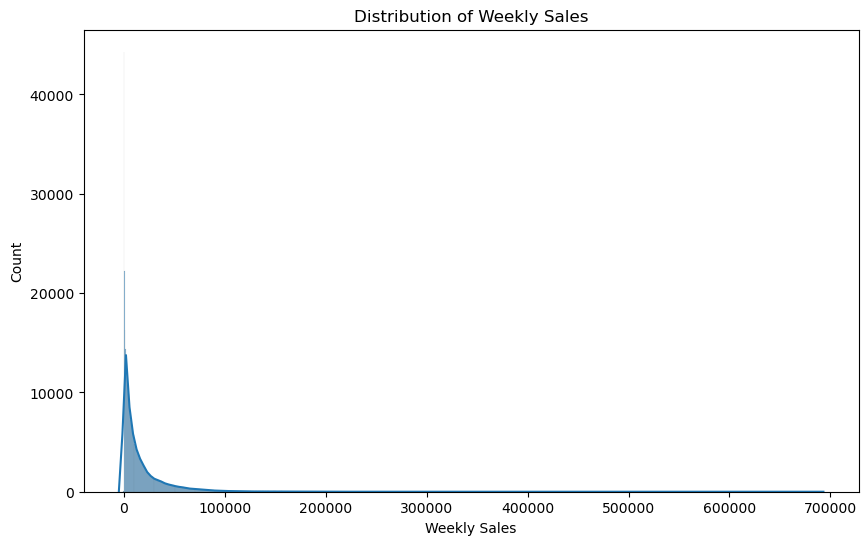
\includegraphics[width=0.8\linewidth]{latex/figures_adarsh/Distribution_Sales .png}
        \caption{Distribution of Weekly Sales Across Stores and Departments}
        \label{fig:weekly_sales_dist}
    \end{figure}
    
    \item \textbf{Test Data}: Designed for model validation, this dataset contains unseen sales data against which predictions are tested. It ensures that forecasting models generalize well beyond the training phase, providing a reliable measure of real-world performance.
    
    \item \textbf{Stores Data}: This dataset offers metadata about individual stores, such as their type (e.g., supercenter or discount store) and physical size. These attributes often influence sales patterns, as larger stores or specific formats may attract different customer behaviors.
    \begin{figure}[h]
        \centering
        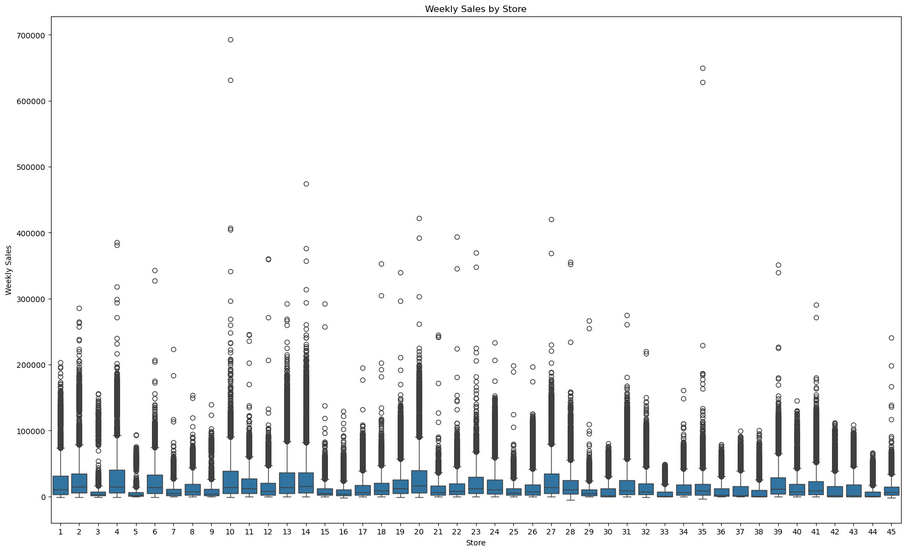
\includegraphics[width=0.8\linewidth]{latex/figures_adarsh/Weekly_Sale_by_Store.png}
        \caption{Comparison of Weekly Sales Across Different Stores}
        \label{fig:sales_by_store}
    \end{figure}
    
    \item \textbf{Features Data}: Encompassing external variables, this dataset includes factors like regional temperature, fuel costs, promotional markdowns, the Consumer Price Index (CPI), and unemployment rates. These elements provide a broader context for sales fluctuations, capturing the impact of environmental and economic conditions on consumer spending.
\end{itemize}

\section{Output Analysis}
The results generated by the forecasting tools offer a window into their effectiveness and practical utility:
\begin{itemize}
    \item \textbf{ARIMA Model Output}: ARIMA’s performance is typically evaluated using metrics like Mean Squared Error (MSE) and Root Mean Squared Error (RMSE). Lower values indicate a closer fit to actual sales data, reflecting higher accuracy. While ARIMA excels with linear trends, it may falter when confronted with intricate, non-linear patterns, limiting its adaptability in diverse retail scenarios.
    \begin{figure}[h]
        \centering
        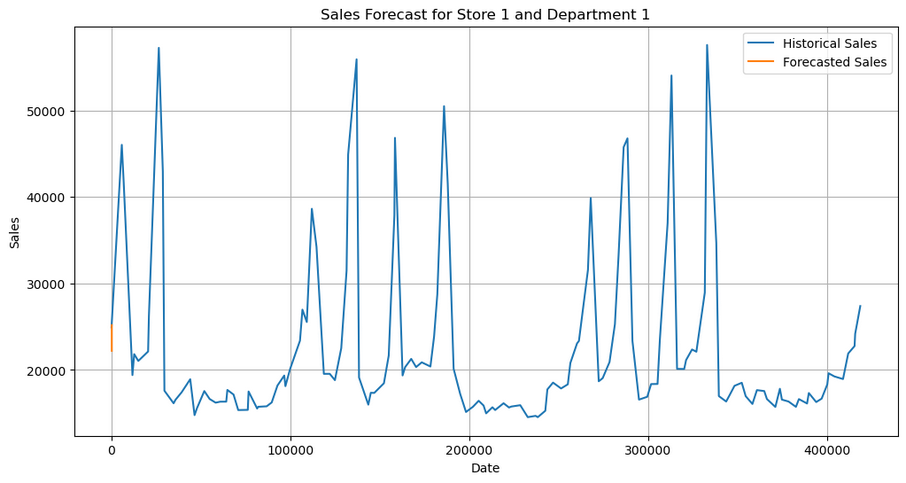
\includegraphics[width=0.8\linewidth]{latex/figures_adarsh/Sales_forecasting.png}
        \caption{Time Series of Weekly Sales with ARIMA Predictions}
        \label{fig:sales_over_time}
    \end{figure}
    
    \item \textbf{XGBoost Model Output}: XGBoost often outperforms traditional models like ARIMA, delivering lower MSE and RMSE scores, especially with voluminous or multifaceted datasets. Its strength lies in its ability to model non-linear relationships and interactions between variables, such as how holiday sales might vary with store size or markdowns, making it a versatile tool for retail forecasting.
    
    \item \textbf{LSTM Model Output}: LSTMs shine in scenarios where sales data exhibits pronounced seasonality or long-term trends. By capturing temporal dependencies—like the lingering effects of a major holiday season—these models produce forecasts that align closely with complex real-world patterns. However, their computational demands and the need for extensive hyperparameter tuning can pose challenges.
    \begin{figure}[h]
        \centering
        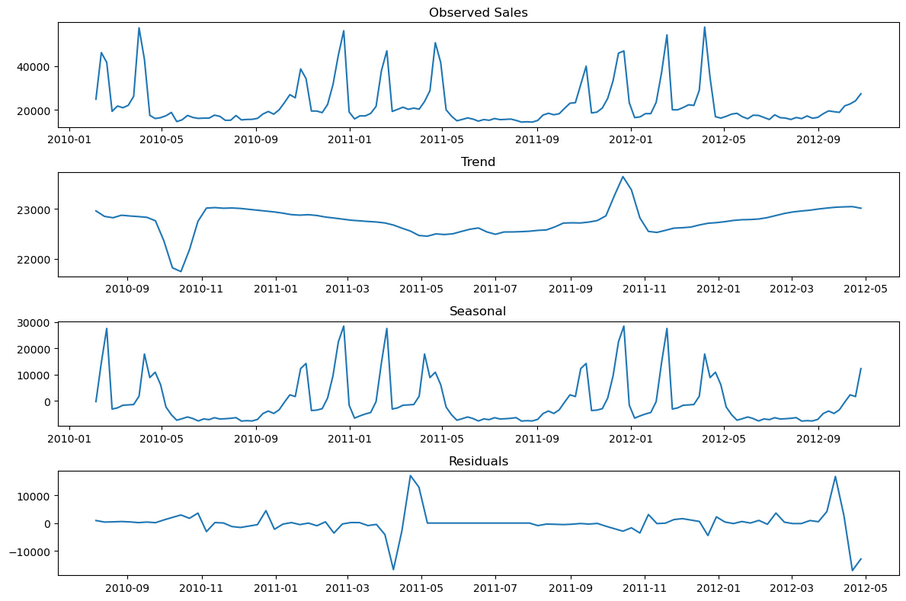
\includegraphics[width=0.8\linewidth]{latex/figures_adarsh/LSTM.png}
        \caption{Predicted Sales for Store 1, Department 1 Using LSTM}
        \label{fig:sales_forecast}
    \end{figure}
\end{itemize}

\section{Detailed Explanation of Tools and Outputs}
\subsection{ARIMA Model}
ARIMA remains a staple in time series forecasting due to its interpretability and effectiveness with straightforward datasets. It operates by analyzing past data to predict future outcomes, assuming a linear relationship between historical and future values.
\begin{itemize}
    \item \textbf{Components of ARIMA}:
    \begin{itemize}
        \item \textit{AR (AutoRegressive)}: Incorporates past sales values to inform predictions, leveraging historical patterns.
        \item \textit{I (Integrated)}: Applies differencing to stabilize the data, removing trends to achieve stationarity.
        \item \textit{MA (Moving Average)}: Accounts for past prediction errors, smoothing out random fluctuations.
    \end{itemize}
    \item \textbf{Limitations}: ARIMA’s reliance on linearity can hinder its performance with datasets featuring multiple seasonal cycles or abrupt shifts, necessitating more advanced alternatives for complex retail environments.
\end{itemize}

\subsection{XGBoost Model}
XGBoost stands out as a high-performance machine learning solution, blending speed with predictive power. It constructs an ensemble of decision trees, iteratively refining predictions to minimize errors.
\begin{itemize}
    \item \textbf{Key Features}:
    \begin{itemize}
        \item \textit{Gradient Boosting}: Combines numerous weak learners into a robust model, enhancing accuracy with each iteration.
        \item \textit{Handling Missing Values}: Automatically manages gaps in data, a common issue in retail datasets, without requiring extensive preprocessing.
        \item \textit{Regularization}: Mitigates overfitting by penalizing overly complex models, ensuring generalizability.
    \end{itemize}
    \item \textbf{Advantages}: Its ability to process non-linear patterns and scale to large datasets makes XGBoost ideal for forecasting in dynamic retail settings.
\end{itemize}

\subsection{LSTM Model}
LSTMs address the limitations of traditional RNNs by preserving information over long sequences, making them a powerful choice for time-dependent data like sales records.
\begin{itemize}
    \item \textbf{Key Features}:
    \begin{itemize}
        \item \textit{Memory Cells}: Store critical information across time steps, enabling the model to recall distant events.
        \item \textit{Gates}: Regulate information flow—input, forget, and output gates decide what to retain or discard, enhancing adaptability.
    \end{itemize}
    \item \textbf{Advantages}: LSTMs excel at detecting subtle temporal relationships, such as gradual shifts in consumer behavior or recurring seasonal effects, though their resource intensity requires careful implementation.
\end{itemize}

\section{Humanized Perspective}
Beyond the technical realm, sales forecasting is about empowering businesses to thrive in a competitive market. Accurate predictions translate into smarter inventory decisions—ensuring shelves are stocked without excess waste—while also informing pricing strategies that balance profitability with customer appeal. For a retailer like Walmart, this means anticipating demand surges during holidays or adjusting stock levels based on regional economic conditions, ultimately enhancing customer satisfaction.

The integration of machine learning elevates this process by weaving in external influences, such as weather forecasts predicting a cold snap that boosts clothing sales, or fuel price hikes that curb discretionary spending. This comprehensive approach equips businesses to navigate uncertainty, seize opportunities, and maintain a strategic edge in an ever-evolving industry.

\section{Discussion}
Selecting the right forecasting tool hinges on the dataset’s characteristics and the task’s demands. ARIMA suits simpler datasets with clear, linear trends—like predictable weekly sales in stable markets—offering a lightweight, interpretable solution. However, when datasets grow complex, incorporating multiple variables like promotions, weather, or store-specific traits, machine learning models like XGBoost or LSTMs become essential.

XGBoost strikes a balance between efficiency and sophistication, making it ideal when computational resources are constrained or rapid deployment is needed. Conversely, LSTMs are better suited for datasets with deep temporal structures, such as sales influenced by annual cycles or multi-year trends, despite their higher resource demands.

The optimal strategy often involves blending these tools—using ARIMA for baseline forecasts, XGBoost for variable-rich scenarios, and LSTMs for time-sensitive insights. By tailoring the approach to the business’s goals and data profile, retailers can sharpen their forecasting precision, driving smarter decisions and operational excellence.